back to the phase shifter today. really want to get this thing working before
the end of the semester. probe impedance seems to matter a distressing amount
for performance —- a 100x probe measures a full 20\textdegree\ more shift.

tried an integrator instead\ldots\ and that was \emph{really} easy to tune and
worked nearly immediately, with basically exactly 90\textdegree\ shift. guess
we're using that!

\begin{figure}[H]
	\centering
	\includegraphics[width=.7\textwidth]{int-shifter-sch.png}
	\caption{the schematic of the integrator-based phase shifter.}
\end{figure}

\begin{figure}[H]
	\centering
	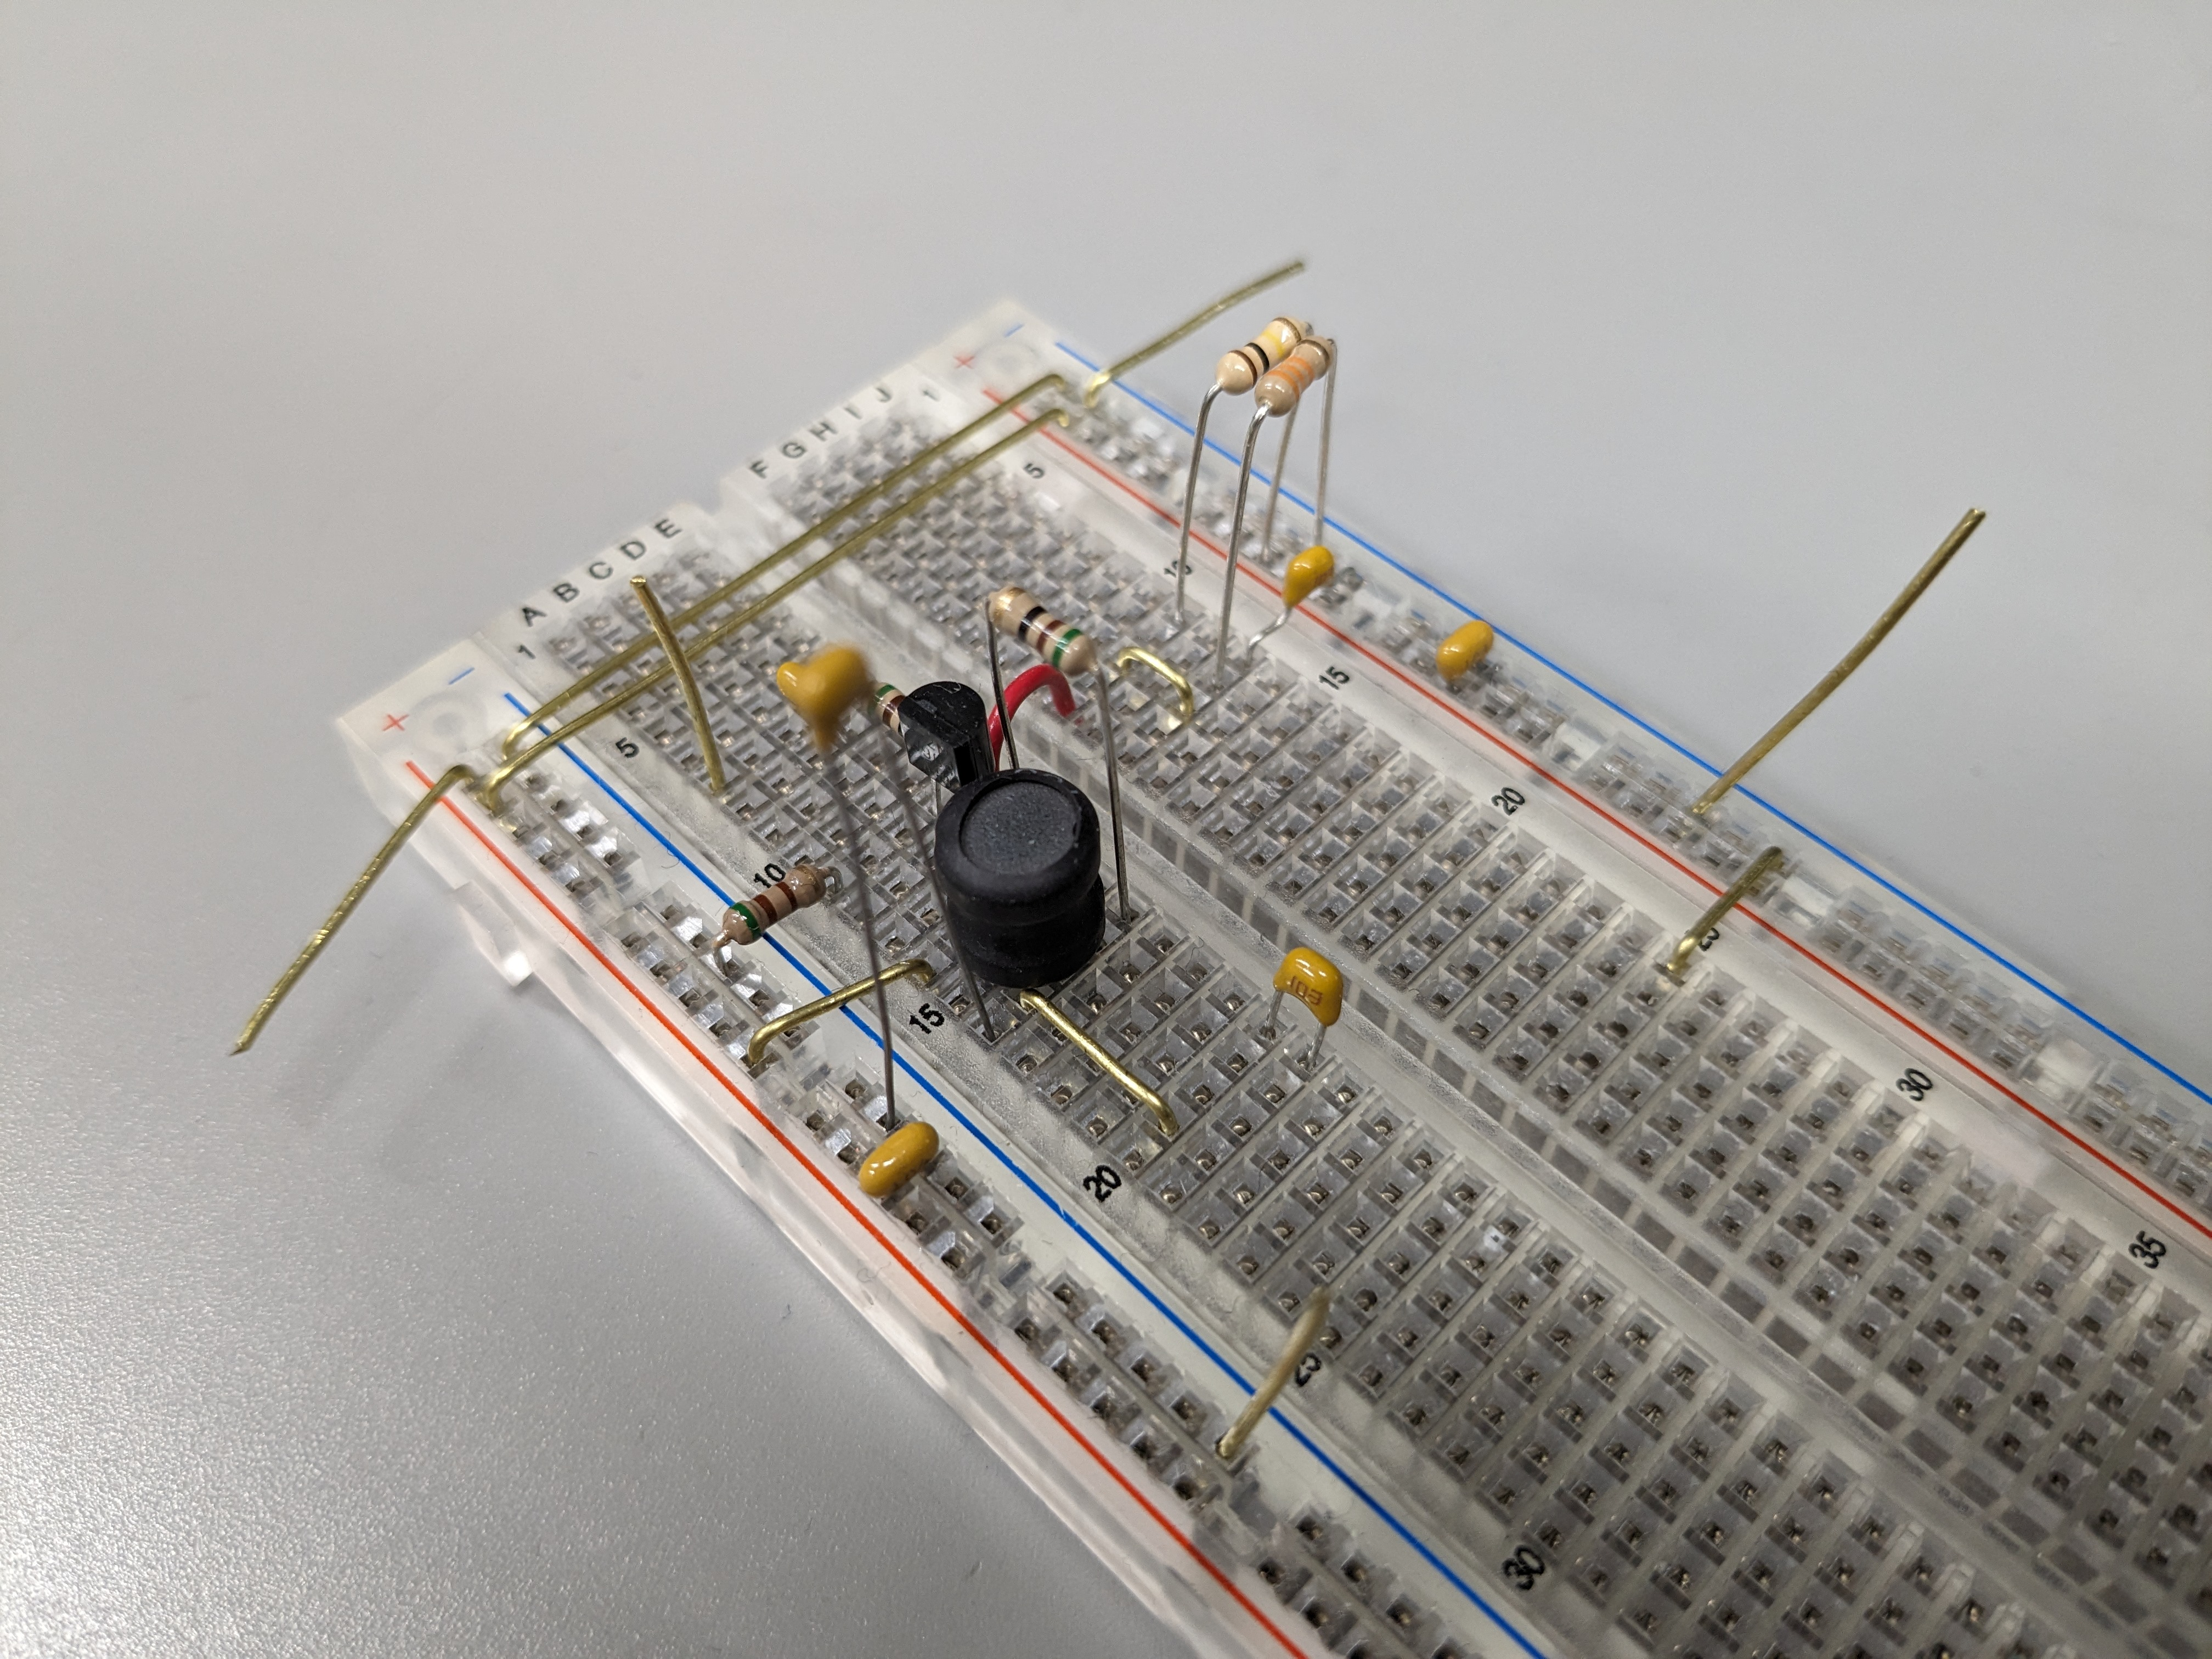
\includegraphics[width=.7\textwidth]{int-shifter-breadboard.png}
	\caption{an implementation of the phase shifter.}
\end{figure}
